\section{Experiments}

Every setting below is one of six: three datasets crossed with the two loss stems, at $n=5$ seeds unless stated. We ask four questions in order --- what produces the separation, whether its one free coefficient can be set without labels, how it compares against label-free post-hoc rotation, and what it costs. Design choices that could have been made differently are tested in Appendix~\ref{app:design}.

\subsection{Data and factors}
\label{sec:data}

We use the synthetic generator of Section~\ref{sec:synthetic} and two public sets, PTB-XL \citep{wagner2020} and HAPT \citep{reyesortiz2016, hapt2015}; Table~\ref{tab:datasets} gives their sizes and their two factors.

\begin{table}[!tb]
\caption{The three datasets. The transient proxy is computed from the signal, never from labels. Channels are 1, 1 (lead II) and 3 (acceleration axes); the grouping unit for splits is 4,812 patients for PTB-XL and 30 subjects for HAPT; chance is 0.333, 0.500 and 0.167.}
\label{tab:datasets}
\centering
\footnotesize
\setlength{\tabcolsep}{4.5pt}
\begin{tabular}{lllllll}
\hline
 & Size & Rate & Patch & Window $L$ & Persistent factor & Transient proxy \\
\hline
Synthetic & $10^6$ steps & --- & 8 steps & 256 & regime $s$, 3-way & OU $u$ \\
PTB-XL & 5,000 rec. & 100\,Hz & 10 (0.1\,s) & 100 (10\,s) & diagnosis, 2-way & voltage \\
HAPT & 2,104 win. & 50\,Hz & 4 (0.08\,s) & 256 (20.5\,s) & activity, 6-way & $\lVert a\rVert$ \\
\hline
\end{tabular}
\end{table}

Splits are per group, patient for PTB-XL and subject for HAPT, and normalization uses training-split statistics only. No data is selected by label before training: HAPT's transition and unlabeled segments, 24.7\% of the total, are excluded from scoring but left in the pre-training input, windows are cut without consulting activity boundaries, and labels are read per position. On PTB-XL the rule that initializes $\tau$ does not apply, since the heartbeat repeats regularly and its autocorrelation oscillates instead of decaying; $\tau$ is set by hand there (Section~\ref{sec:limits}).

\subsection{What creates the separation}
\label{sec:ablation}

We switch each of the two devices we add --- the horizon gate and the cross-covariance penalty --- on and off. The mechanism-free cell (Section~\ref{sec:xcov}) is the baseline in which only the coordinate split remains.

\begin{table}[!tb]
\caption{Separation index by mechanism. Cells are SEP, $n=5$ seeds, $\lambda=4$; bold marks the best cell in each row.}
\label{tab:ablation}
\centering
\small
\begin{tabular}{llcccc}
\hline
Dataset & Stem & Neither & Gate only & xcov only & \textbf{Gate + xcov} \\
\hline
Synthetic & Reg & 0.135 & 0.342 & 0.279 & \textbf{0.408} \\
Synthetic & NCE & 0.121 & 0.124 & 0.488 & \textbf{0.749} \\
PTB-XL & Reg & 0.375 & 0.404 & 0.312 & \textbf{0.495} \\
PTB-XL & NCE & 0.392 & 0.503 & 0.283 & \textbf{0.567} \\
HAPT & Reg & 0.521 & 0.537 & 0.236 & \textbf{0.632} \\
HAPT & NCE & 0.297 & 0.366 & 0.162 & \textbf{0.515} \\
\hline
\end{tabular}
\end{table}

In Table~\ref{tab:ablation} the model with both devices ranks first in all six settings, and neither device alone reaches that value. On the contrastive stem of the synthetic data the gate alone is indistinguishable from the mechanism-free case (0.124 against 0.121), yet adding that same gate to the penalty raises SEP from 0.488 to 0.749: the two devices need each other. The penalty alone is actively harmful on the real data, breaking down the inclusion term and falling below even the mechanism-free case.

The ``Neither'' cells take the first 16 of the 64 dimensions, and their SEP agrees in all six settings to within 0.015 with the SEP of 16 dimensions drawn at random from the same embedding. Without our devices, any part of the embedding holds the two factors to a similar degree, so coordinate position carries no meaning by itself; our contribution is to give those coordinates structure. Fig.~\ref{fig:embed} shows the same contrast qualitatively.

\begin{figure}[!tb]
\centering
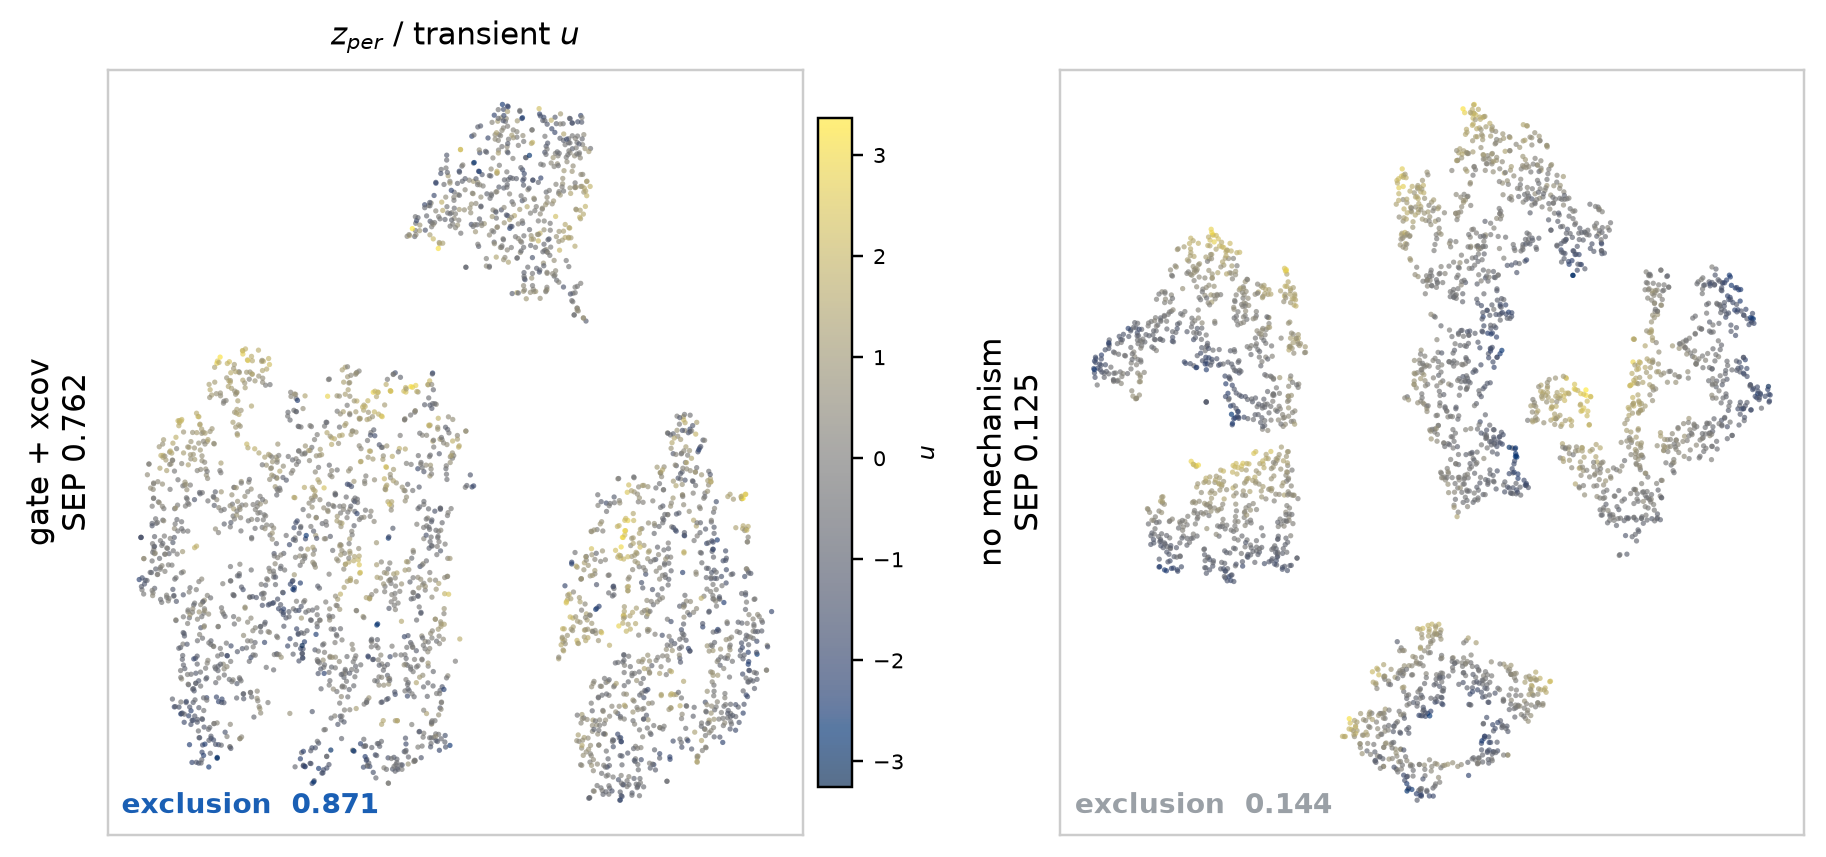
\includegraphics[width=0.86\textwidth]{figs/fig_embed_exclusion.png}
\caption{The exclusion term, seen directly: a t-SNE of $\zslow$ coloured by the transient factor, with the mechanism and without it. This is the only one of the three terms that differs between the two models --- inclusion is \numFigInclusion{} against \numFigNoInclusion{} and allocation \numFigAllocation{} against \numFigNoAllocation. All six panels are in Fig.~\ref{fig:embed_full}.}
\label{fig:embed}
\end{figure}

Three further design choices could each have gone the other way, and none of them is left to argument. Replacing the smooth gate with a step at $\tau$, gating $\zslow$ symmetrically as well, and predicting the raw signal instead of a latent target are each tested in Appendix~\ref{app:design}; all three are worse, and the latent target by a factor of two.

\subsection{Setting the penalty weight without labels}
\label{sec:lambdafree}

$\lambda$ was chosen by looking at downstream performance, which makes ``our best $\lambda$ separates well'' partly circular. We therefore define a criterion that uses no task label at all, the \textbf{purity--persistence score}: $\zslow$ should be \emph{pure}, holding none of the transient factor, and \emph{persistent}, still predicting its own value far ahead.
\begin{equation}
\mathrm{PPS} = \underbrace{\big[1-s_{\text{tra}}(z^{\mathrm{per}})\big]_0^1}_{\text{purity}} \cdot
    \underbrace{s_{\text{self}}(z^{\mathrm{per}};\,\Delta>\tau)}_{\text{persistence}},
\label{eq:pps}
\end{equation}
Purity is one minus the transient proxy's score from $\zslow$ --- the exclusion term of Eq.~\ref{eq:sep}, and the proxy is computed from the signal. Persistence is how well $\zslow$ predicts \emph{its own} value more than $\tau$ ahead; neither the labels nor the target encoder enters. The product is required because each half alone has a degenerate maximum: an empty block is perfectly pure, a constant block is perfectly self-predicting, and multiplying kills both.

\caption{Choosing $\lambda$ without labels. \emph{PPS}: the
$\lambda$ our label-free criterion picks; \emph{oracle}: the $\lambda$ maximizing SEP, which
does use labels; \emph{margin}: the gap between the top two $\mathrm{PPS}$ values, where
small is not confident agreement. $n=3$ seeds.}
\label{tab:lambdafree}
\centering
\footnotesize
\setlength{\tabcolsep}{3pt}
\begin{tabular}{lccc}
\hline
Setting & PPS & Oracle & Margin \\
\hline
Synth. / Reg & 1 & 1 & 0.234 \\
Synth. / NCE & 16 & 16 & 0.111 \\
PTB-XL / Reg & 4 & 4 & 0.023 \\
PTB-XL / NCE & 4 & 4 & 0.004 \\
HAPT / Reg & 1 & 1 & 0.016 \\
HAPT / NCE & 64 & 64 & 0.009 \\
\hline
\end{tabular}


Selecting $\lambda$ by $\mathrm{PPS}$ reproduces the label-selected value in all six settings (Table~\ref{tab:lambdafree}). On synthetic data the criterion is also doing real work rather than agreeing by luck: purity alone would have chosen $\lambda=\numJexclOnlyLam$, close to the worst choice by the oracle (SEP \numJexclOnlySep{} against \numJbestSep{} at $\lambda=\numJbestLam$), and it is the persistence half, collapsing from \numJlongBest{} to \numJlongCollapse{} once $\lambda\ge4$, that rules it out. A collapse monitor would not have caught this: effective rank \emph{rises} from \numJrankLo{} to \numJrankHi{} over the same range, so the penalty is not emptying $\zslow$ but scattering it along the time axis.

The margin between the top two $\mathrm{PPS}$ values is \numJmarginSynthLo--\numJmarginSynthHi{} on synthetic but only \numJmarginRealLo--\numJmarginRealHi{} on the real sets, and we did not store its seed-level spread, so the four real-data agreements are not distinguishable from chance at this sample size. The honest reading is that the criterion is verified on synthetic data, consistent on real data, and cheap to run wherever the transient proxy exists.

\subsection{Against label-free post-hoc rotation}
\label{sec:rotation}

If an embedding trained without the gate is rotated post-hoc without labels --- by principal component analysis, by slowness-ordered independent component analysis, or by slow feature analysis (SFA) --- does it reach the same separation? These methods need no horizon gate at all, so they are the sharpest objection to our method.

We have one knob and the post-hoc rotations have none, so we report the whole curve rather than a single point (Fig.~\ref{fig:rotation}). On the synthetic data the curve passes above every post-hoc rotation point, and principal component analysis fails completely (SEP \numSynthPca) --- direct evidence that a ranking by variance is not a ranking by persistence, since the transient factor crowds into the leading components and nothing is left in the complement. On the real data we do not lead. The verdict over all six settings is three wins to three losses, but split apart it is two of two on synthetic and three losses of four on real data, with losing margins of \numRealLossLo--\numRealLossHi{} against a winning margin of 0.099.

\begin{figure}[!tb]
\centering
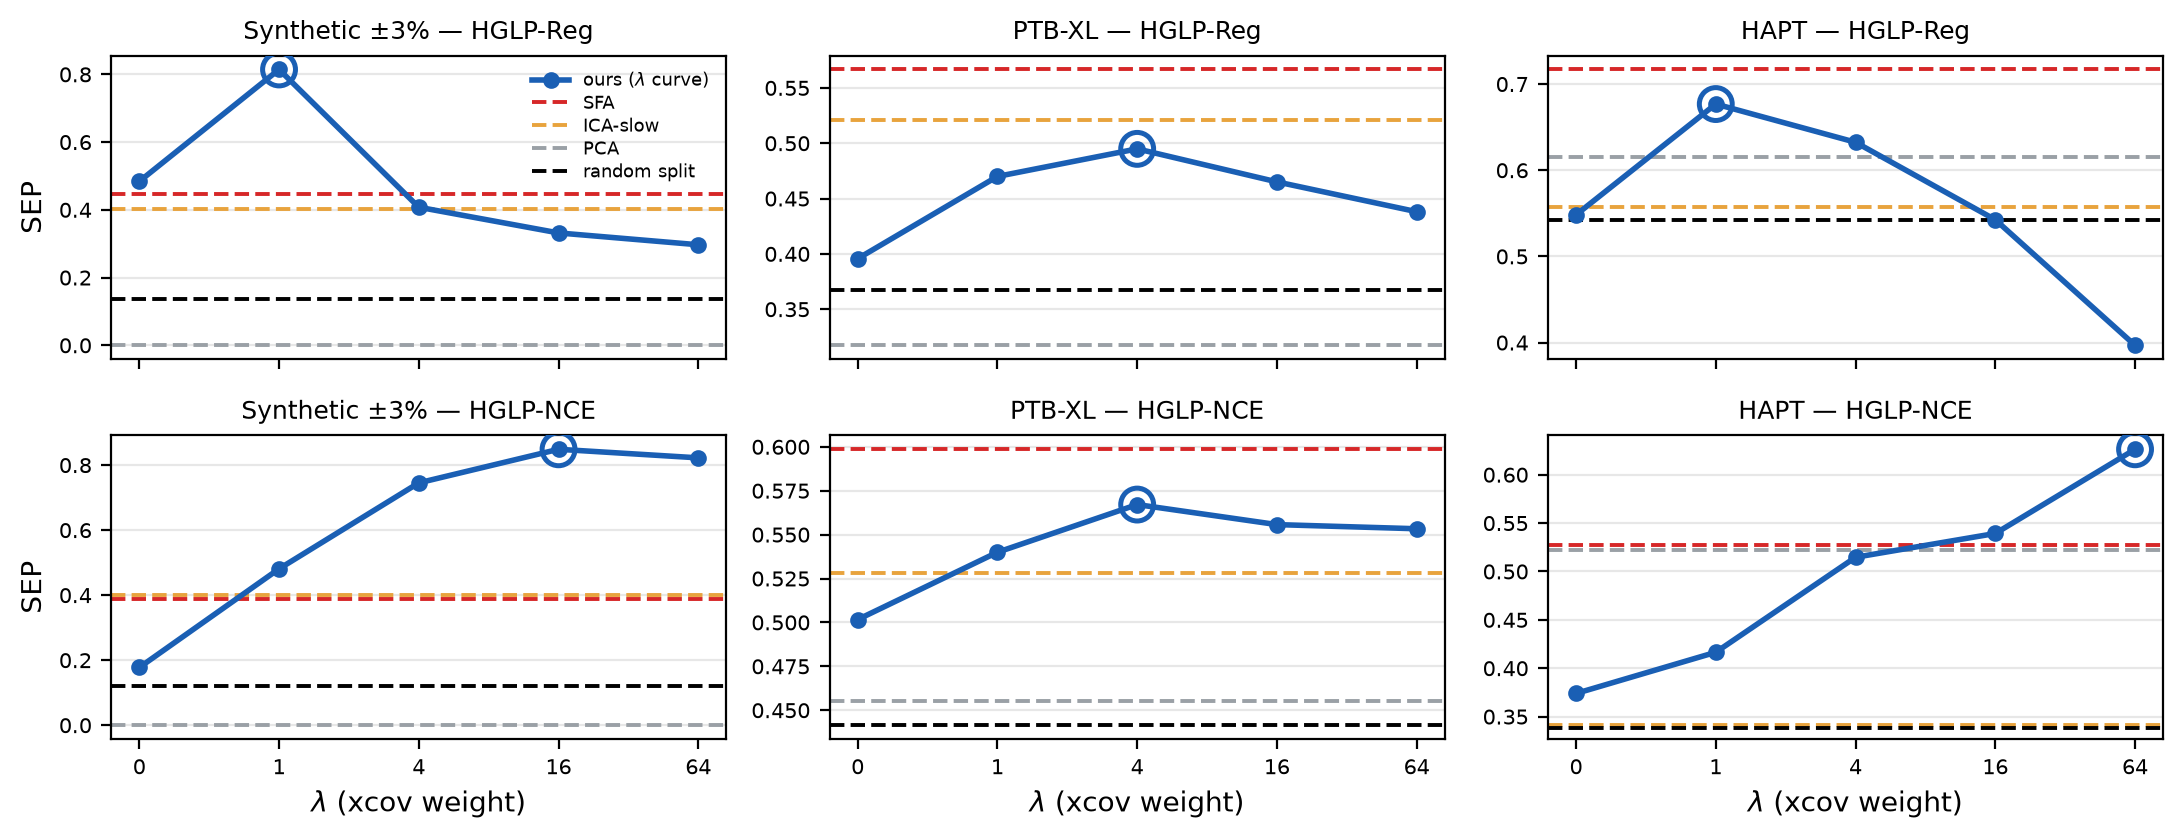
\includegraphics[width=0.92\textwidth]{figs/fig_rotation_sep.png}
\caption{SEP against the penalty weight $\lambda$, $n=5$ seeds. Our method traces a curve with its best point ringed; each post-hoc unmixing has no knob and is a horizontal line. A win is our curve rising above the SFA line.}
\label{fig:rotation}
\end{figure}

\paragraph{Where the shortfall sits.}
SEP is a product of three factors, so a single number cannot say which one is losing. Splitting it and pairing by seed gives an unusually clean answer (Appendix~\ref{app:probe}, Table~\ref{tab:terms}): inclusion is a draw in all six settings ($\numInclDiffLo$ to $\numInclDiffHi$), \textbf{every real-data loss is a loss on exclusion alone}, and every win is a win on allocation. The method does not degrade diffusely; it degrades on the one term the objective was never able to enforce (Section~\ref{sec:gate}).

\paragraph{The exclusion we do achieve is a linear-level one.}
Every probe so far has been linear, and an unreadable direction is not the same as an absent one. Holding the features, the splits and the blocks fixed and replacing only the reading head with a one-hidden-layer MLP --- given equally to SFA, PCA and ICA --- exactly one term collapses, and it is exclusion: averaged over four methods and four real settings, inclusion moves $\numMlpIncl$ and allocation $\numMlpAlloc$, while exclusion falls $\numMlpExcl$ and as much as $\numMlpExclWorst$ in the worst row. The transient information is still present in $\zslow$; the linear probe could not reach it. Our claim therefore narrows to a linear-level one --- and the diagnosis above is not an artifact of weak probing, since SFA's lead on exclusion survives the stronger head and in places widens, while PCA and ICA degrade sharply. Appendix~\ref{app:probe} gives the per-setting values and the caveats.

\paragraph{Why SFA leads where it leads.}
The explanation is that persistence and slowness mostly coincide on real data. On PTB-XL this is plain: the diagnosis is constant within a record, so its time derivative is zero, which is the limiting solution of the quantity SFA maximizes. On HAPT it is not constant within a window and we did not measure why the coincidence holds there, so that half of the explanation remains untested. What the synthetic data shows is the other side of the same statement: built so that the persistent factor is neither constant within a window nor present in the slow band, it is the one dataset on which the post-hoc route fails. What remains ours is that the coordinates are fixed during training, so no second fitting stage is needed at deployment --- an operational difference, not a difference in the quality of the separation.

\subsection{The cost of separation, and stability under domain shift}
\label{sec:cost}

Measured against the full embedding of a mechanism-free model --- not against our own $z_{\mathrm{full}}$, which would mix in the effect of block width --- the downstream cost of using $\zslow$ alone is effectively zero on synthetic data and PTB-XL, and $-0.111$ macro-F1 on HAPT (regression stem; $-0.072$ contrastive). HAPT is the only dataset whose persistent factor is not constant within the window: 57\% of its windows straddle an activity transition, which is also why its cost is the one that shows.

We then carry a probe fitted on clean data with few labels into a domain where the transient factor has been perturbed by a gain, $x \mapsto x\cdot(1+s)$ up to $s=2$ --- a bijection that leaves the persistent labels legible (HAPT activities survive at macro-F1 0.696, chance 0.167). The effect is small and mostly inside the noise. At 25 labels on HAPT/Reg the gated block's drop is 0.113 smaller than a width-matched mechanism-free block's, five times the seed standard deviation; in the other five settings the effect lies inside the noise, and 17 of 24 cells are negative by sign alone (Table~\ref{tab:shift}). Nowhere does absolute performance overtake the mechanism-free model. HAPT is at once the dataset with the largest cost and the only one with a visible shift effect: the gate buys a smaller drop and pays for it in absolute performance.

\begin{table}[!tb]
\caption{Degradation under domain shift. Each cell is the gated block's drop in macro-F1 from the clean domain to the most perturbed one, minus the same drop for a width-matched mechanism-free block; paired by seed, $n=5$. Negative means it degrades less --- \textbf{it never overtakes in absolute terms}.}
\label{tab:shift}
\centering
\small
\begin{tabular}{lccc}
\hline
Setting & 25 labels & 100 labels & All labels \\
\hline
\textbf{HAPT / Reg} & $\mathbf{-0.113}\pm$\textbf{0.023} & $\mathbf{-0.096}\pm$\textbf{0.029} & $-0.053$$\pm$0.056 \\
HAPT / NCE & $-0.017$$\pm$0.072 & $+0.015$$\pm$0.012 & $+0.007$$\pm$0.016 \\
PTB-XL / Reg & $-0.044$$\pm$0.048 & $-0.033$$\pm$0.048 & $-0.024$$\pm$0.035 \\
PTB-XL / NCE & $-0.036$$\pm$0.032 & $-0.010$$\pm$0.024 & $-0.009$$\pm$0.024 \\
Synthetic / Reg & $-0.012$$\pm$0.102 & $+0.043$$\pm$0.099 & $+0.064$$\pm$0.077 \\
Synthetic / NCE & $-0.044$$\pm$0.069 & $-0.055$$\pm$0.054 & $-0.045$$\pm$0.055 \\
\hline
\end{tabular}
\end{table}
